
\chapter{Validation}
\section{Validation Strategy}
Model validation could be considered an important step towards creating a robust and useful simulation tool. A greater volume of literature is availalbe for the validation of Ray based methods such as~\cite{Ahnert2005,Tsingos2002,Foteinou2010}, and the validation of a hybrid scheme by Southern \textit{et al} is available ~\cite{Southern2013}. Studies such as Hill~\cite{Hill2012} incorporate validation as a subset of a greater work. This section will review the results of simulations using the FDTD and PSTD tools described above, with a small 3D domain and different excitation signals. The validation of these simulation tools will be in proving that wave propagation is occurring with reasonable spectral accuracy.\\

\subsection{The Domain}
The domain used was a fully bounded rectangular room with the following properties:\\

\begin{itemize}
\item Length $L_x = 5m$
\item Width $L_x = 4m$
\item Height $L_z = 3m$
\item Volume = $ v = 60m^3$
\item Surface Area $S_{area} = 94m^2$
\item Uniform Absorption Coefficient $\alpha = 0.45 $
\item Schroeder Frequency  $f_{schroeder} = 107Hz $,
\item The Reflection Order $N_{reflections} = 30.7$
\item Mean Free Path Between Reflections $MFP = 2.55m$
\item Eyring Reverberation Time $RT_{60} = 0.1719s $
\end{itemize}

The theoretical room mode frequencies below the Schroeder frequency are shown below:\\
\begin{figure}[H]
\centering
  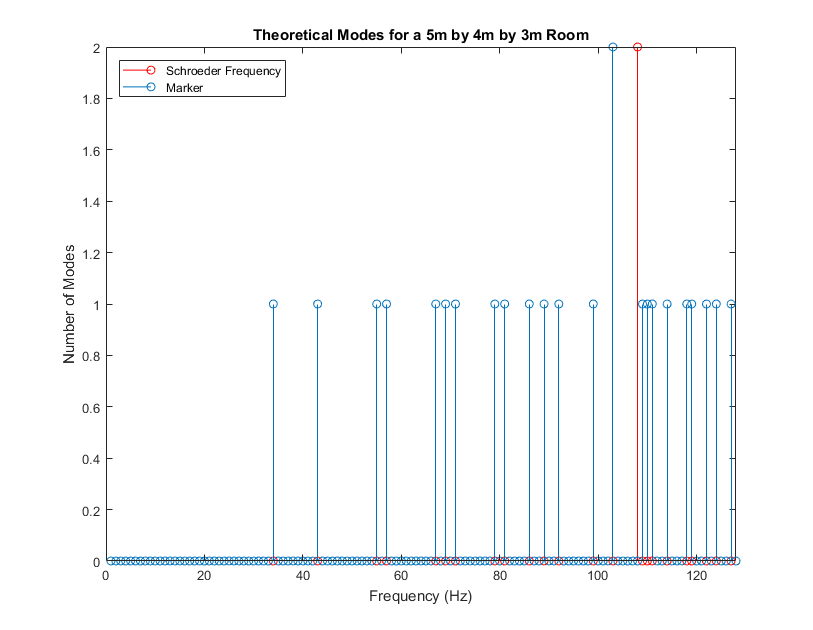
\includegraphics[width=\textwidth]{./graphics/modesuptoschr.png}
  \caption{Room Modes up to Schroeder Frequency for a Small Rectangular Room}
\end{figure}

The source position was $1.0m$ in each direction from a bottom cornerl. Five receiver positions were recorded, one quater on the x and y dimensions from each corner, all at the middle of the domain on the z axis. The source type was a soft source as described earlier in this doccument. Two source signals were implemented in seperate simulations; an MLS sequence of 11th order with 2 repetitions, and a $1kHz$ tone burst signal containing three pulses of 10 cycles with a gap of equal length to the bursts. The MLS signal was generated using the MLS toolbox by Mark Thomas~\cite{Mrt2008}, and the tone-burst was generated using tools in the Matlab DSP Systems toolbox. The signals were normalised with a Gaussian window to the length of the signals. The windowing of the MLS signal should minimise instability caused by discontinuity of the source term. The smoothing of the tone bursts with a window should cause the spectral bandwidth of the signal to be wider than the tone frequency, sharing cues for spectral shift. The maximum frequency of interest in this validation was $5kHz$, giving a $0.333e^{-5}s$ step time for the FDTD and SFDTD simulation, and a $0.1e^{-4}s$ step time for the PSTD simulation.

\section{Results}
The aim of the simulations was be to show that the models propagate pressure waves with minimal error in the average power spectral density between source and receiver location. Frequency domain averaging of the source and receiver location signals was undertaken using Matlab pwelch function. This function uses Welch's overlapping segment averaging estimator to average a series of discrete Fourier transforms, creating a smoothed average frequency response over the course of the signal without transforming the whole signal in one go~\cite{Welch1967}.

\subsection{FDTD Simulation Results}

\begin{figure}[H]
\centering
\textbf{Results of FDTD Simulation With Windowed MLS Signal}
  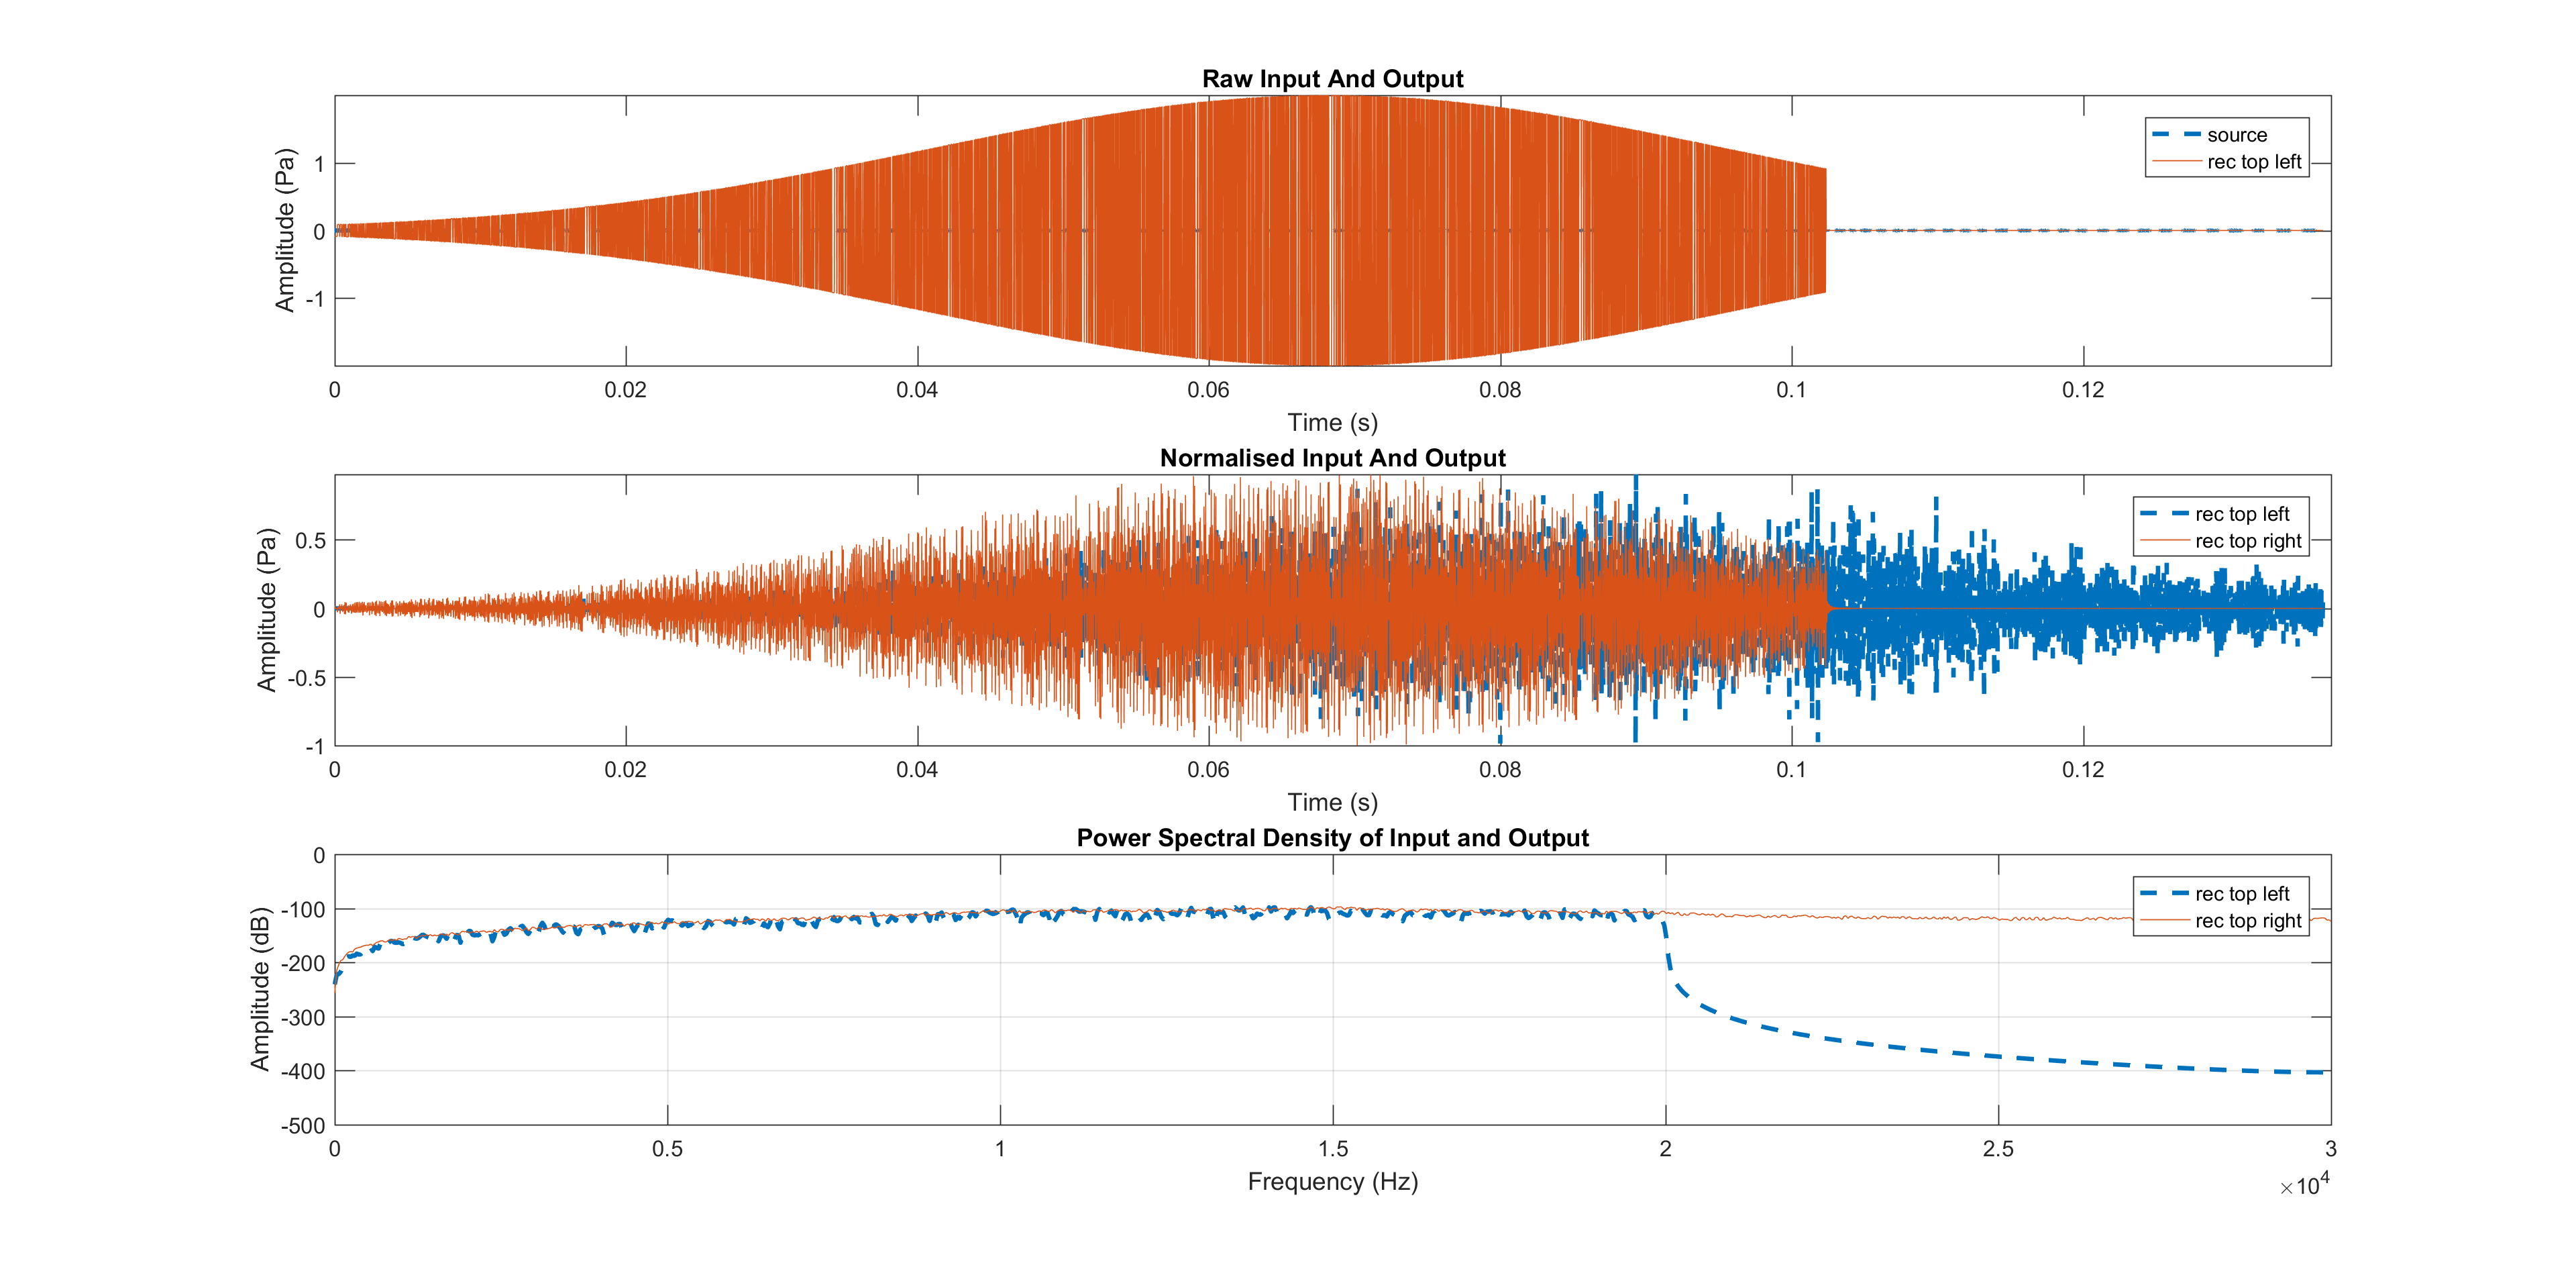
\includegraphics[width=\textwidth]{./graphics/FDTDvalidationFinal.png}
  \caption{FDTD Simulation Data With Windowed MLS Source With 10kHz Maximum Frequency}
  \end{figure}
  \begin{figure}[H]
\centering
  \textbf{Results of FDTD Simulation With Three Windowed 1kHz Tone Bursts}
  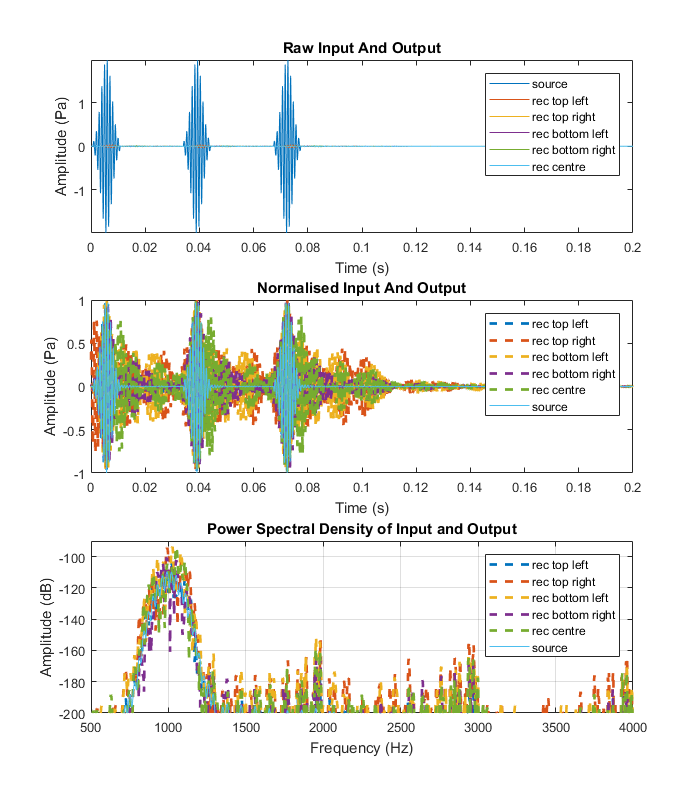
\includegraphics[width=\textwidth]{./graphics/FDTDtoneburst1k.png}
  \caption{FDTD Simulation Data With Windowed Tone Burst Source With 2kHz Maximum Frequency}
\end{figure}

The results of the simulation with and MLS stimulus show that although a maximum frequency of interest of 10kHz was accounted for, signal content up to 20kHz is visible in the spectrum analysis. MLS is a pseudo-random signal with a 'flat' frequency response that is determined by the sampling frequency of the simulation, the resolution of the stimulus in the frequency domain is determined by the order of the MLS signal which in this case is $2^{11}$. In the time domain analysis of the signal, the two signals are shifted and overlaid to account for the delay of propagation, and there is clearly some decaying reverberation present after the the stimulus has finished, showing that the reflecting boundaries are working. The spectrum of the response is smoothed, and the scale of the plot and smoothing caused by the use of pwelch masks room mode effects. An FFT of the reciever signal may show evidence of room modes and the receiver position.


\subsection{SFDTD Simulation Results}

\begin{figure}[H]
\centering
\textbf{Results of SFDTD Simulation With Windowed MLS Signal}
  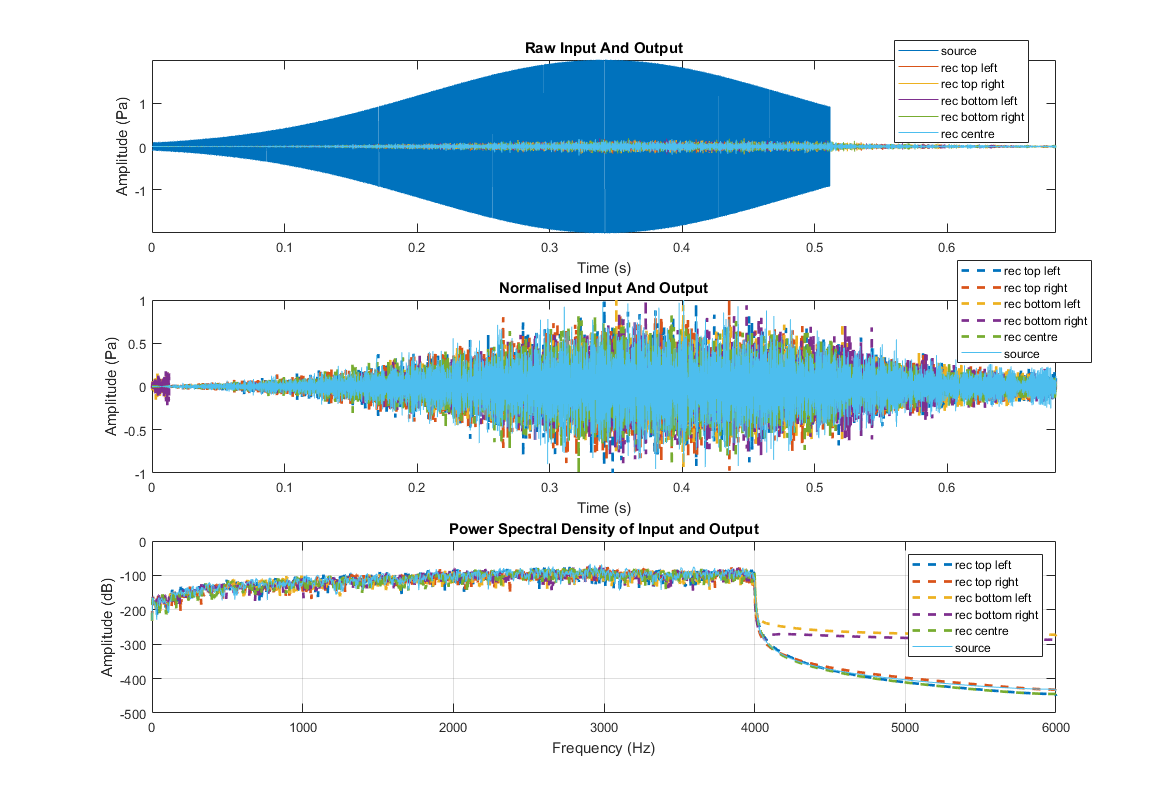
\includegraphics[width=\textwidth]{./graphics/sfdtdMLS.png}
  \caption{SFDTD Simulation Data With Windowed MLS Source With 2kHz Maximum Frequency}
  \end{figure}
  \begin{figure}[H]
\centering
  \textbf{Results of SFDTD Simulation With Three Windowed 1kHz Tone Bursts}
  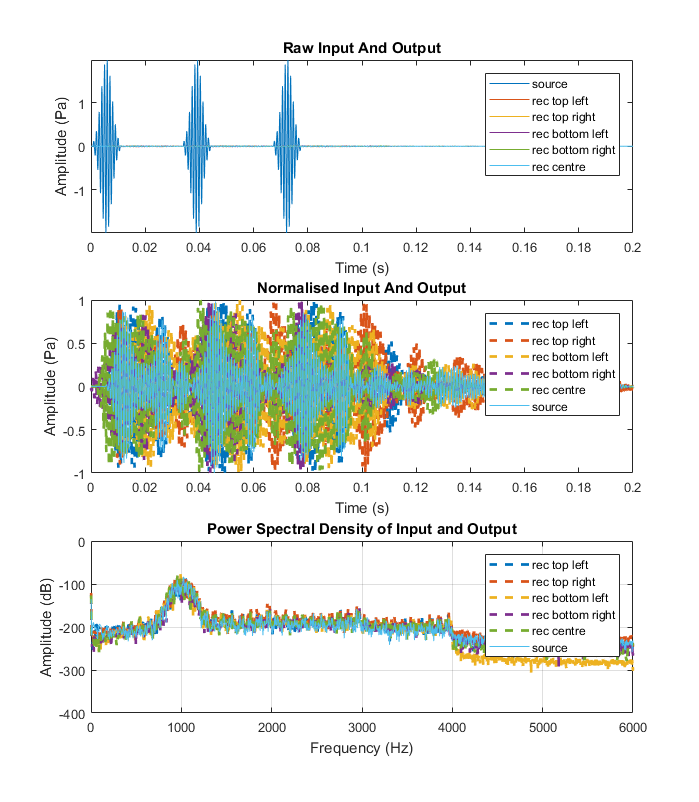
\includegraphics[width=\textwidth]{./graphics/SFDTDvalidationTB.png}
  \caption{SFDTD Simulation Data With Windowed Tone Burst Source With 2kHz Maximum Frequency}
\end{figure}

Due to time constraints with running simulations the SFDTD simulations were completed with a maximum defined frequency of 2kHz, and both sets of simulation data show signal content up to 4kHz which is similar to the content scaling of the FDTD simulation. The simulation with windowed  MLS shows that the frequency content of the signal rolled off at low frequency but was predominantly flat, which is also similar to the FDTD simulation. The time domain results of the simulation with tone bursts shows the system is performing with reverberation and decay, this shows that the boundaries are performing as expected as well as the windowing function with regards to allowing many wave-fronts to propagate. In the spectral analysis of the resultant waveforms, the position and bandwidth of the system signal is similar to the results given by the FDTD model. This shows that the SFDTD method is working appropriately when compared to the FDTD model, with respect to acoustic performance.

\subsection{PSTD Simulation Results}
\begin{figure}[H]
\centering
\textbf{PSTD Validation MLS Data}
  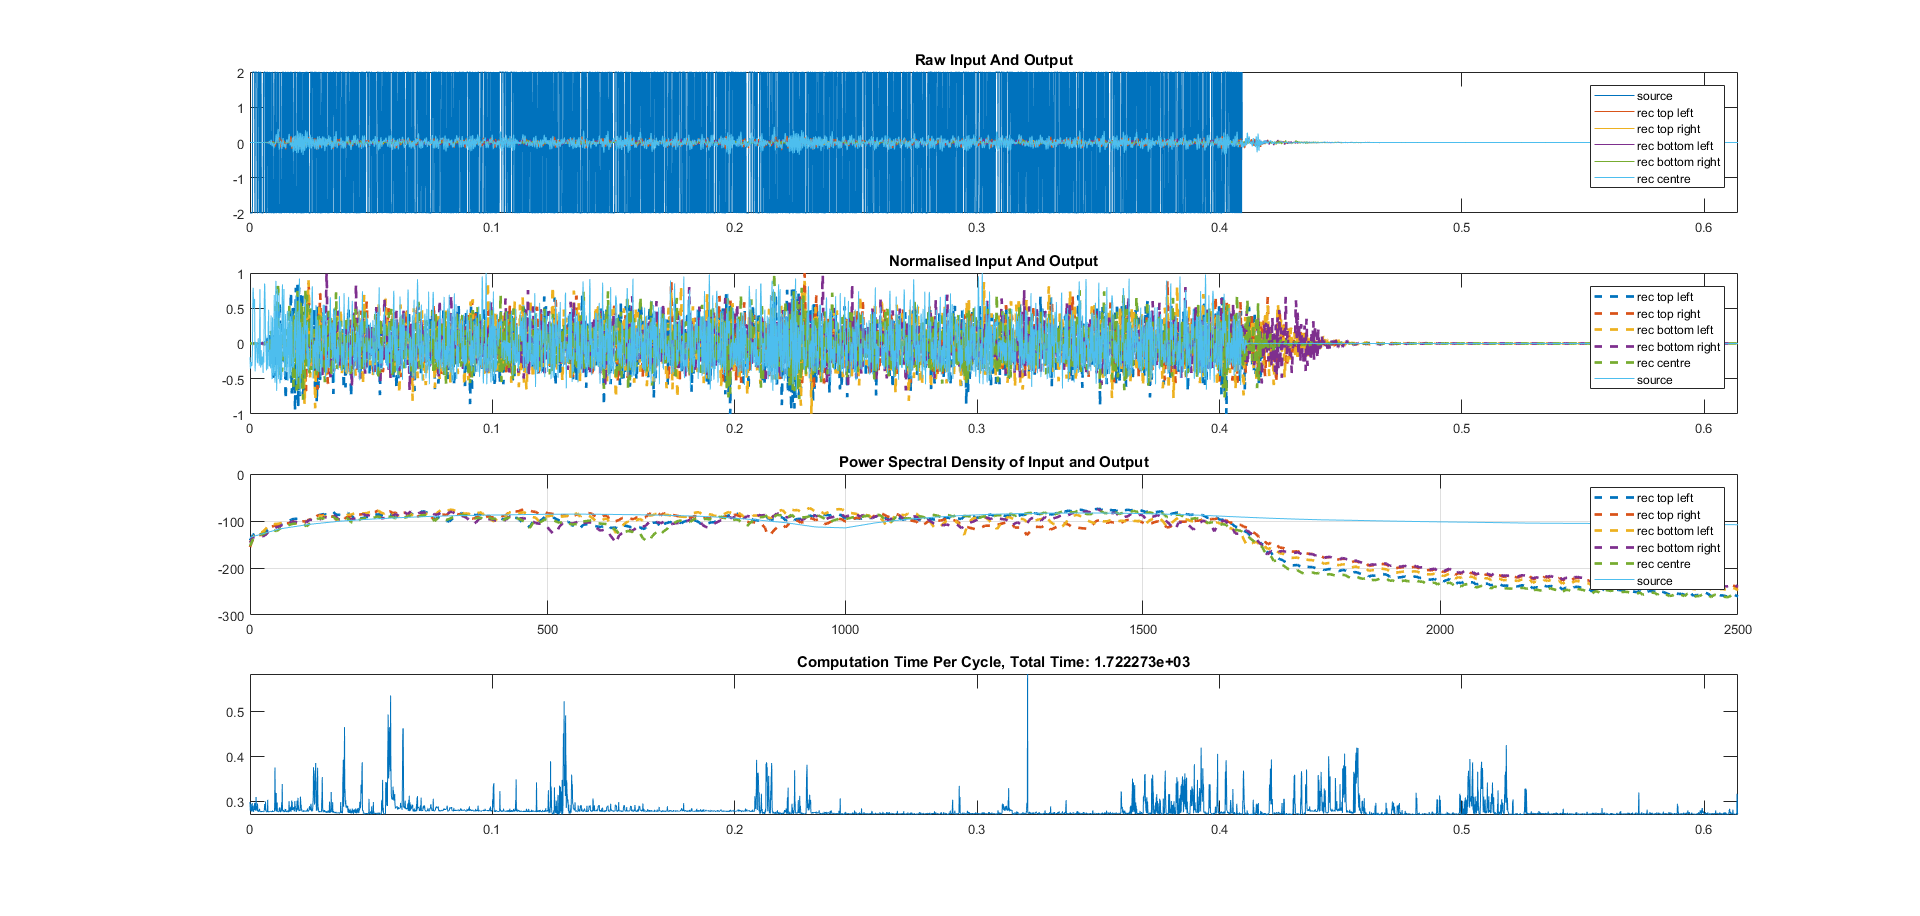
\includegraphics[width=\textwidth]{./graphics/PSTDvalidationFinal.png}
  \caption{Validation data of PSTD simulation With MLS Source}
  \end{figure}
  \begin{figure}[H]
  \centering
  \textbf{PSTD Validation Tone Burst Data}
  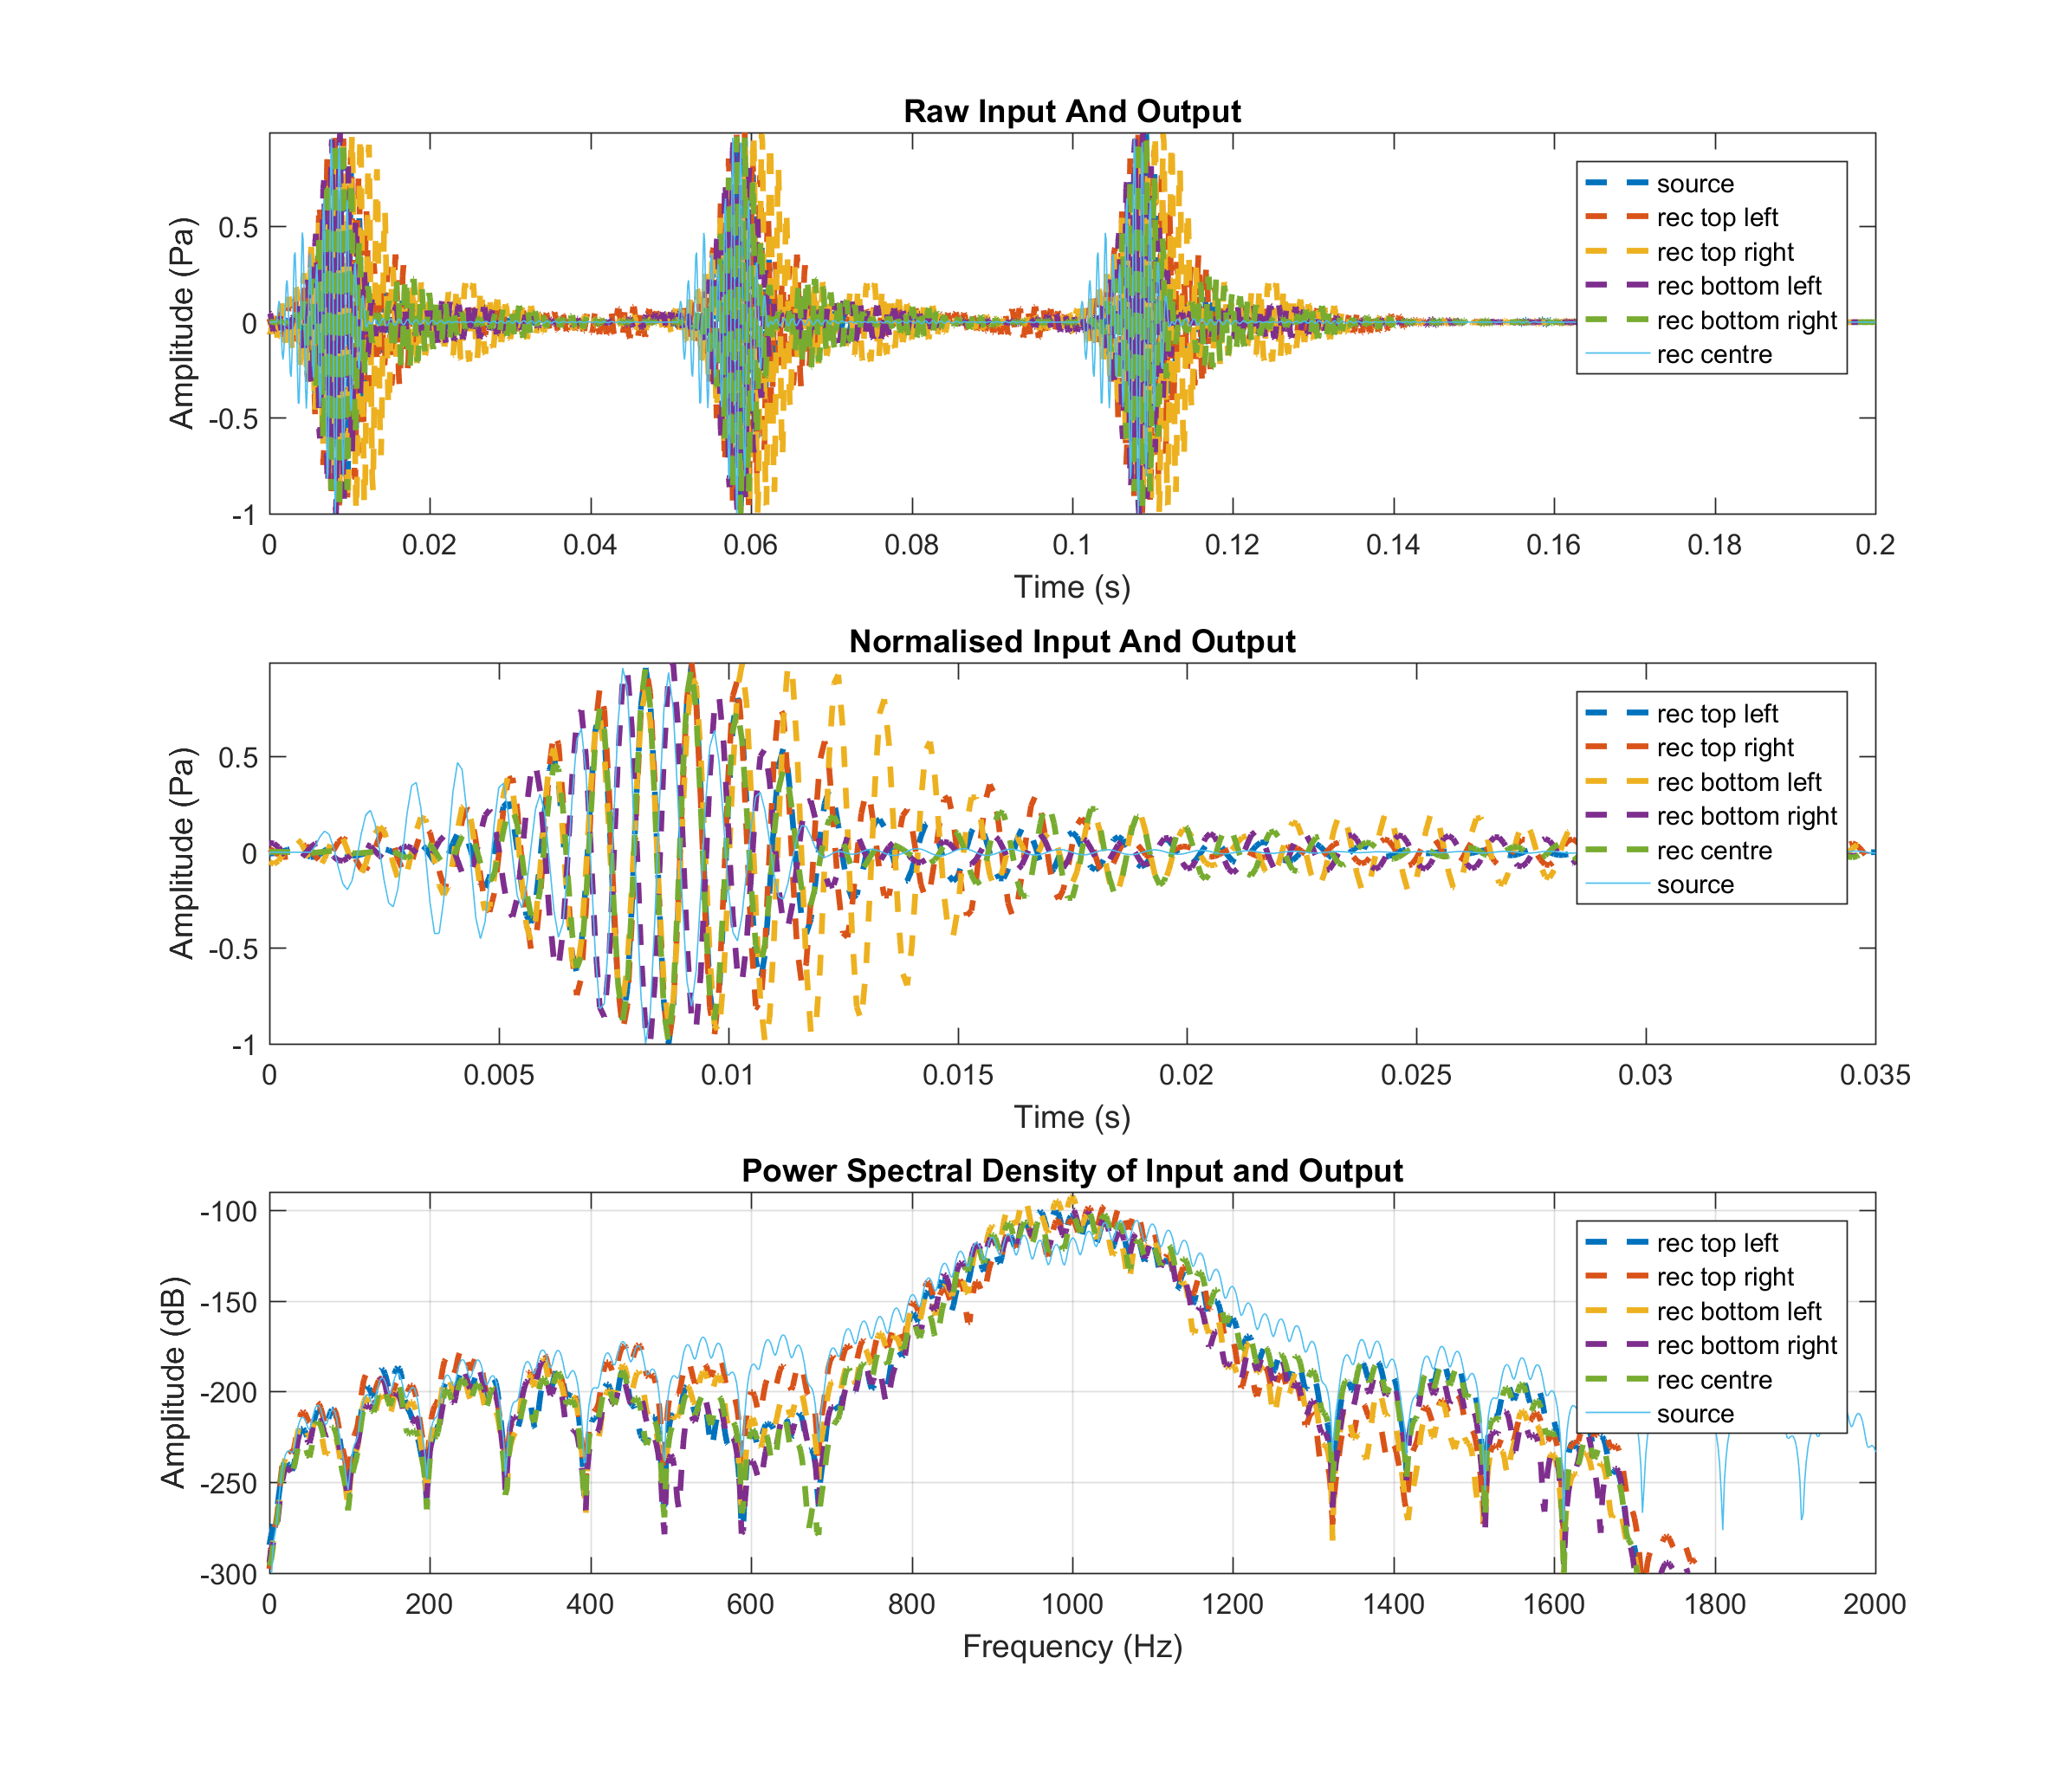
\includegraphics[width=\textwidth]{./graphics/PSTDvalidationFinalTB.png}
  \caption{Validation data of PSTD simulation With Tone Burst Source}
\end{figure}

It can be seen in the spectral analysis of the simulations with an MLS stimulus that the PSTD method shares reasonably good agreement with the FDTD and SFDTD methods around the target frequency, with a slight low frequency roll-off and a generally flat frequency response. The time domain plot of the simulation with a tone-burst stimulus shows quite a large error in the decay response between different positions in the domain. Further to this, considerable comb filtering is present in the spectral analysis of the response. There is also an earlier high frequency roll off in the noise floor than may have been expected when reviewing the MLS simulation results. If the close plot of the time domain data of the simulation with the tone burst is observed, it appears that the wave speed at different positions in the domain is different i.e. parts of the signal speed up and slow down, the modulating effect could be a partial cause of the comb-filtering of the signal. However, the 1kHz band tone is clearly visible as higher than the noise floor of the simulation, suggesting that the performance may be adequate for the purpose of performing an execution speed test.

\subsection{Compared Spectral Analysis for Simulation Results With Tone Burst Stimulus}
Below is a plot of the spatially averaged (average of the receivers), temporal average frequency domain content of the simulations with tone burst stimulus for all three calculation methods:\\

  \begin{figure}[H]
\centering
  \textbf{Spatially Averaged Power Spectral Density of Simulation Input and Mean Output for FDTD, SFDTD and PSTD with 1kHz Windowed Tone Burst Stimulus}
  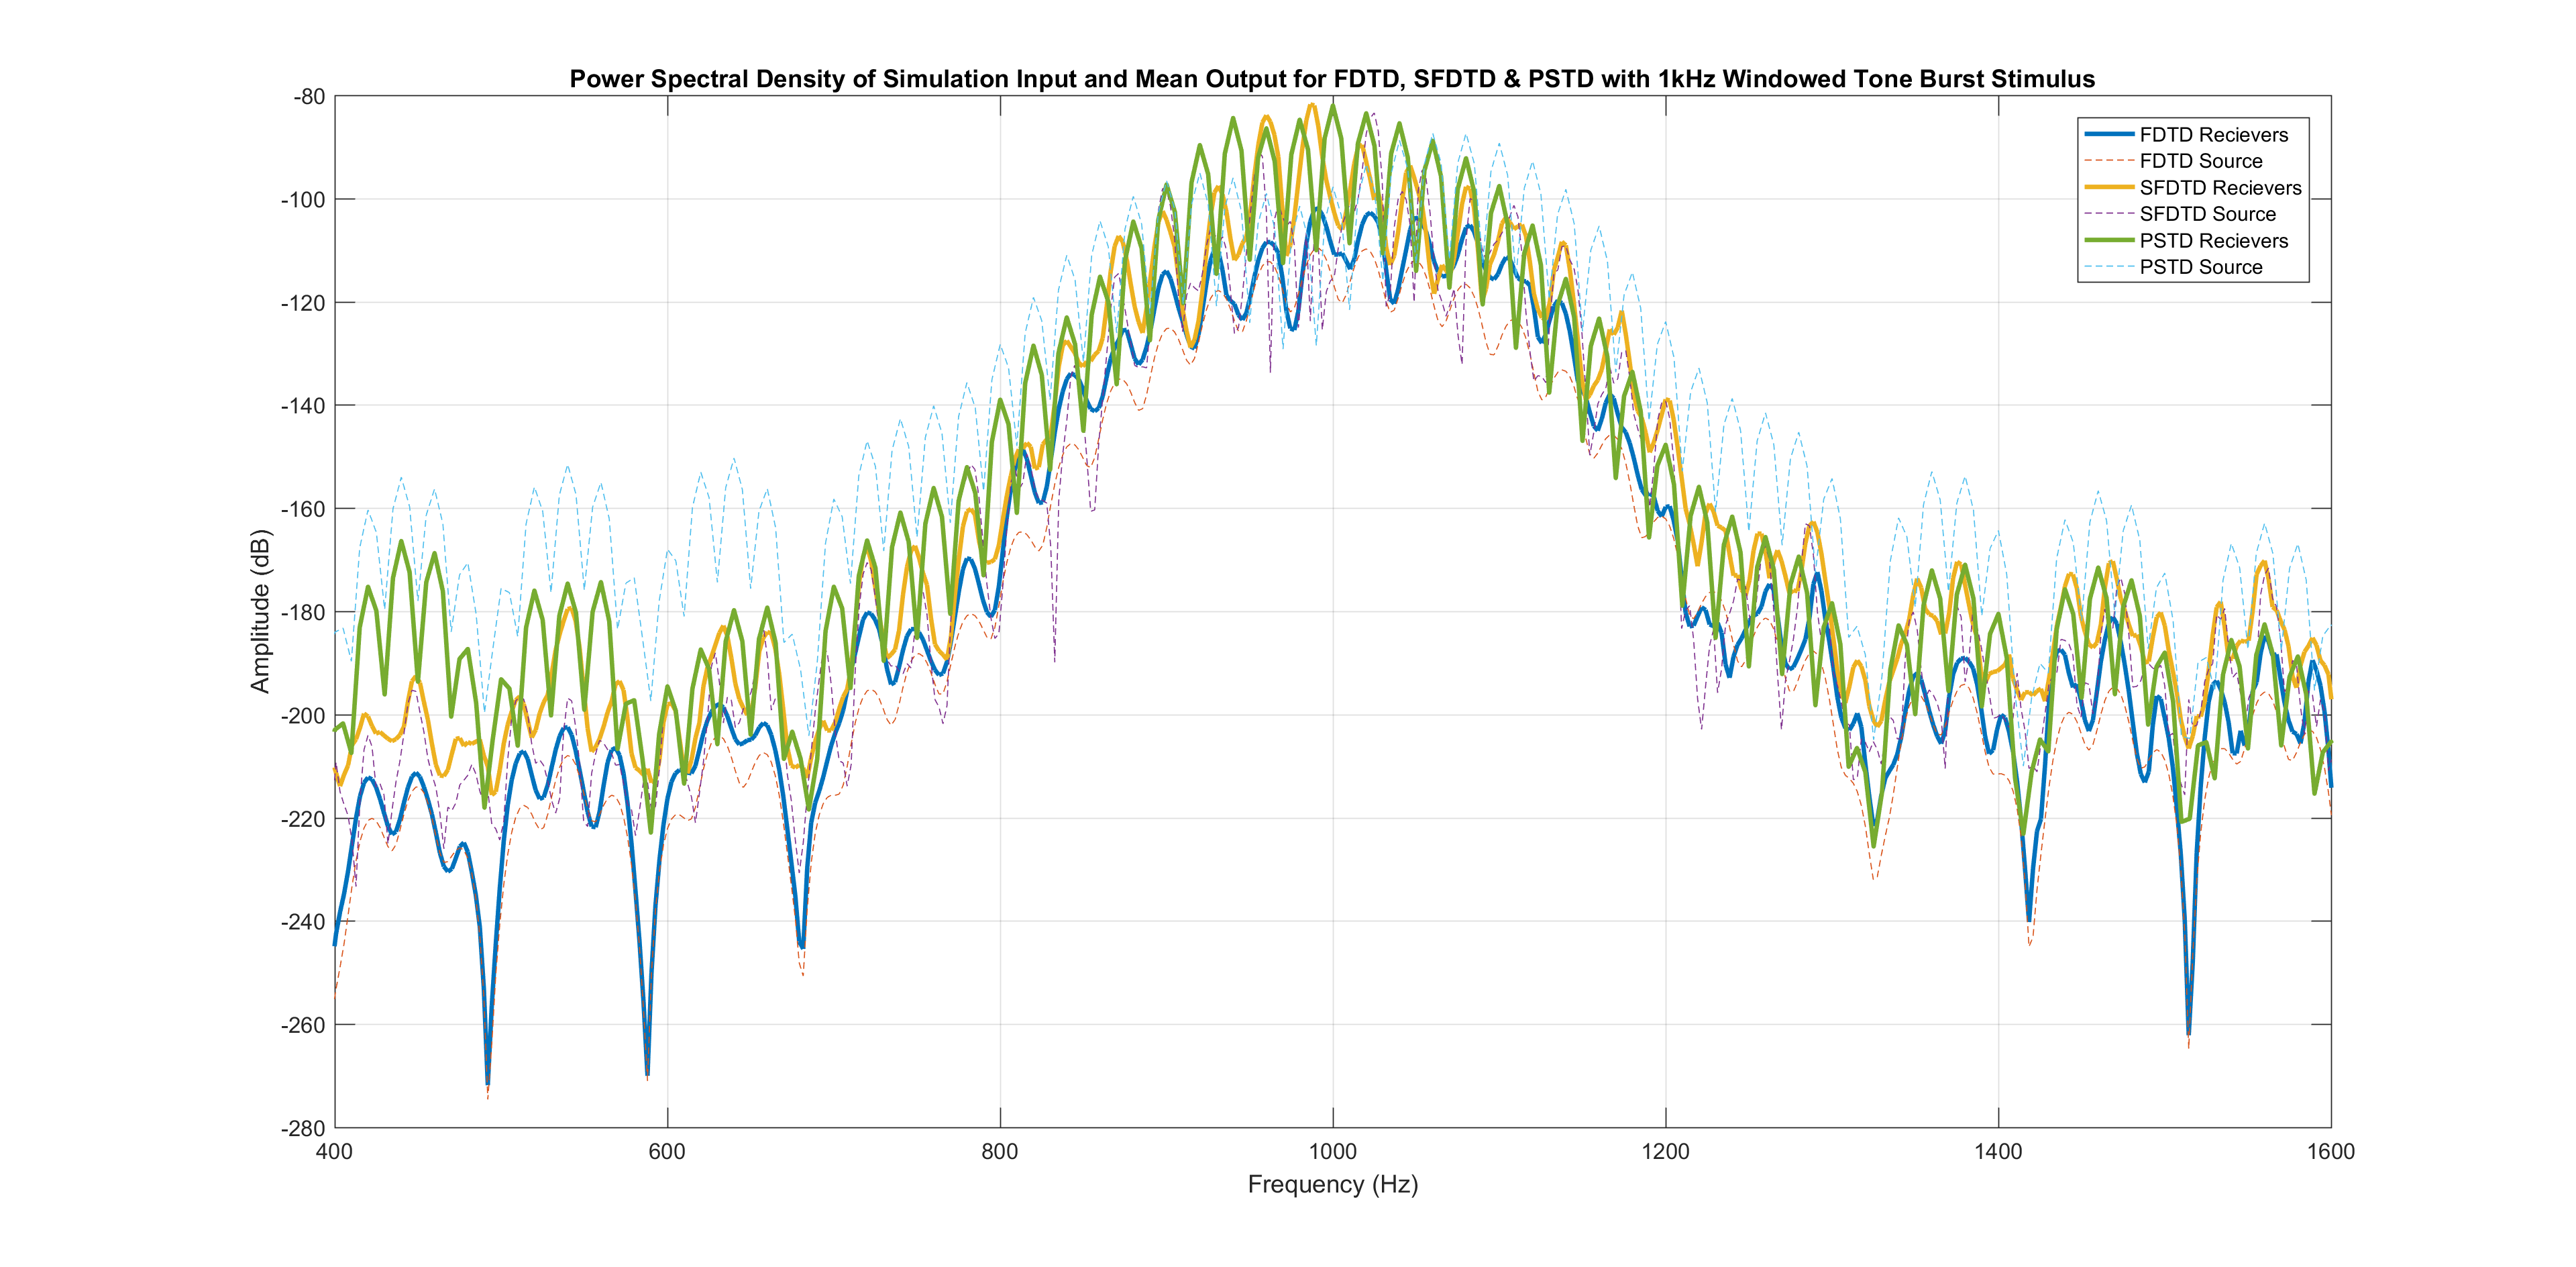
\includegraphics[width=\textwidth]{./graphics/winTBval.png}
  \caption{Averaged spectral content around tone burst frequency for all three methods}
\end{figure}

For any of the three methods to have distinct error in terms of wave propagation compared to the other two methods, it may be expected that the above figure would show a distinct difference in the width of the function around the centre frequency. The results show reasonable similarity, including a uniform dip around $1.3kHz$, $700Hz$ and $500Hz$ that may suggest some similar modal interaction is occurring.

